\section{Motivation}
\label{sec:motivation}

Typically, in communications systems designs, the system is almost always built to account for the characteristics of the propagation medium. In this section, we motivate the design of the RoXOR protocol in the context of wireless interference channels, channels in which the dominant impairment is caused by co-channel interference from other contending users in the network.  

\begin{figure}[t]
\label{fig:collision}
\centering
\vspace*{-0.1in}
\subfigure[Case1] {
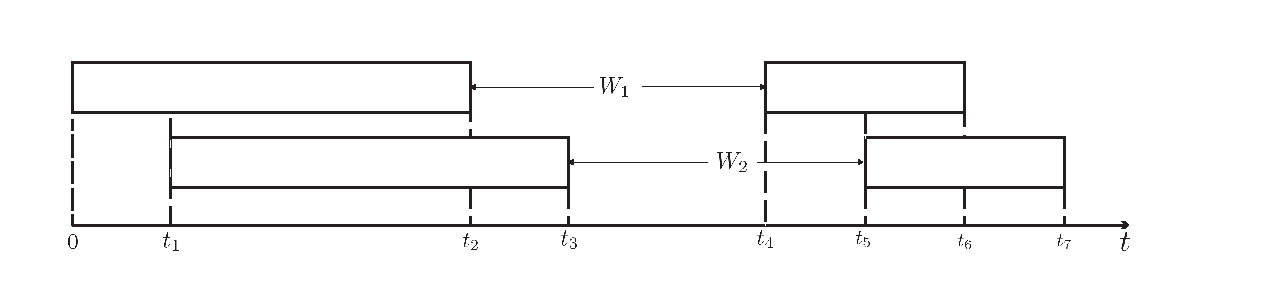
\includegraphics[width=.9\columnwidth]{./figs/roxor_timing_diagram_case1.pdf}
\label{fig:collision1}
}
\subfigure[Case2] {
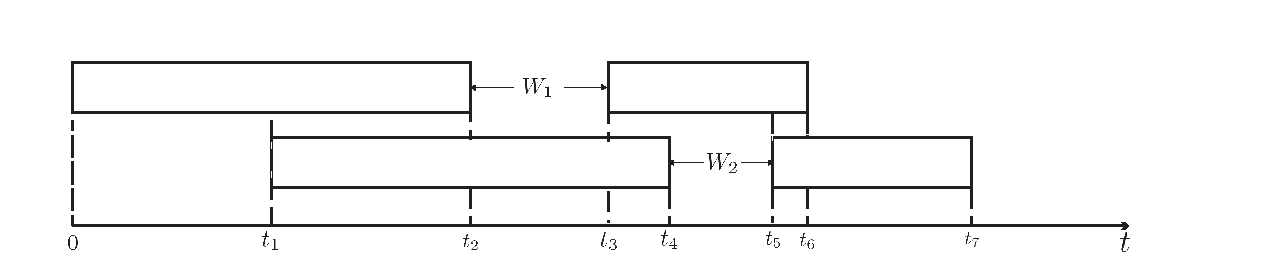
\includegraphics[width=.9\columnwidth]{./figs/roxor_timing_diagram_case2.pdf}
\label{fig:collision2}
}
\subfigure[Case3] {
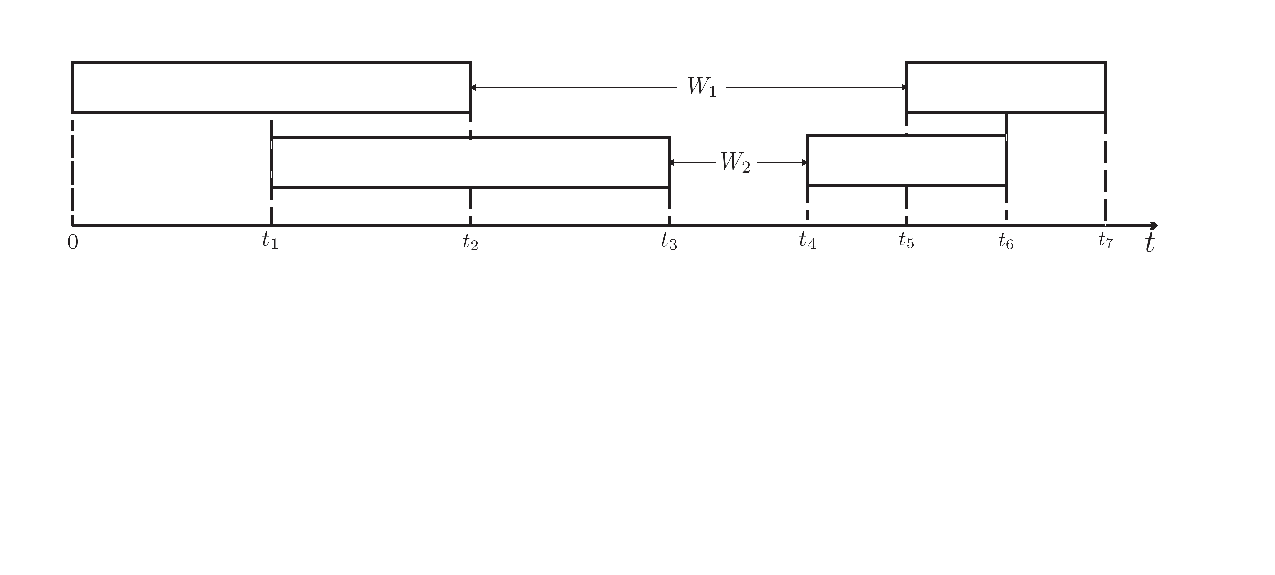
\includegraphics[width=.9\columnwidth]{./figs/roxor_timing_diagram_case3.pdf}
\label{fig:collision3}
}
\vskip -0.5em
\caption{Collision Between Two Packets}
\vskip -1em
\end{figure}

\subsection{Channel Model}
\label{sec:ChModel}
The assumed channel model is such that the errors caused by co-channel interference as shown by figure~\ref{fig:collision1} dominate the number of errors due to random noise. Hence, other effects such as additive noise are not considered because the system is assumed to be operating at sufficiently high SNR. 

Furthermore, we assume that the channel interference is sparse and bursty. Because the interference is intermittent it really does not make sense to use a stronger forward error correction (FEC) 100\% of the time in anticipation of sparse interference events that only occur a fraction of the time. Therefore, an (H)ARQ-like scheme based on re-transmissions would be most suitable to handle the assumed channel impairments.

\subsection{ARQ}
\label{sec: arq}



\subsection{SiC and Decodability}
\label{sec:sic_equations}
When packets of length $L$ from $N$ users collide, applying successive interference cancellation is equivalent to solving a number of equations and finding $LN$ unknowns. Subsequently, for the case of $k$ retransmissions, the minimum number of equations received by the $k^{th}$ retransmission is $(k+1)L$ and the maximum number is $(k+1)LN$.
\begin{equation}
\label{eq:numeq}
(k+1)L \leq N_e \leq (k+1)LN
\end{equation}
Clearly, the amount of equations received after the $k^{th}$ transmission is largely dependent on the overlap between desired and interfering signals. On the other hand, the number of independent equations is related to the structure of the incremental redundancy. Therefore, the key to an effective incremental redundancy scheme is a structure that can maximize the number of independent equations received following each re-transmission.

\subsection{Decodability for Two-Users}
\label{sec:two-user}
As an example, we first look at the decodability for the situation illustrated in figure~\ref{fig:collision1}. First, we define the fractional overlap $\alpha$ and amount of incremental redundancy $\beta$ for packets of size $L$. Both parameters $\alpha$ and $\beta$ are specified as ratios relative to the size of the transmitted packet; hence, $0\leq\alpha\leq1$ and $0\leq\beta\leq1$. For this case, there are two regions in which overlap occur (i.e. at intervals $T_1\in[t_1,t_2]$ and $T_2\in[t_5,t_6]$), and will be denoted $\alpha_1$ and $\alpha_2$ respectively. Therefore, after the first re-transmission, the number of equations $N_e$ becomes
\begin{equation}
\label{eq:Ne1}
N_e = (2L)-(\alpha_1 L)+(2\beta L)-(\alpha_2\beta L)
\end{equation}
Subsequently, the condition required to successfully decode the original packet after the first-retransmission is:
\begin{equation}
N_e \geq 2L
\end{equation}
\begin{equation}
(2-\alpha_1)L + (2-\alpha_2)\beta L \geq 2L
\end{equation}
which eventually gives the following condition on the amount of incremental redundancy $\beta$ required for decodability:
\begin{equation}
\beta \geq \frac{\alpha_1}{2-\alpha_2}
\end{equation}
Further, for an initial overlap of $\alpha_1$, and $\alpha_2=0$, the required incremental redundancy is $\beta \geq \frac{\alpha_1}{2}$, which is reasonable because if both users send $\frac{\alpha_1}{4}$ worth of incremental redundancy, assuming no overlap on re-transmission, this becomes sufficient to decode. Eventually, this establishes the fact that it could be excessive to re-transmit the entire packet (i.e. $\beta=1$) for an initial overlap of $\alpha_1=0.25$. 

\subsection{Incremental Redundancy}
\label{sec:IncRed}

In a protocol that is based on retransmissions, a key parameter is the amount of information
or incremental redundancy $\beta$, that should be sent for each retransmission. A second key parameter is how this information should be encoded. Previously, we discussed how changing the amount of incremental redundancy effects the decodability, now we talk about the structure of such a code.

Consider a block of $k$ information bits, $x^k=\{x_1x_2\dots x_k\}$ that are input into an encoder which results in a code block of size $n$ with code bits denoted $c^n=\{c_1c_2\dots c_n\}$. We say that the degree of code bit $c_m$, where $1 \leq m \leq n$ is $d$ if $c_m$ is composed of a linear combination of $d$ unique terms. In other words:
\begin{equation}
c_m=x_{m_1}\oplus x_{m_2} \oplus \dots \oplus x_{m_d}
\end{equation}

In these terms, the standard ARQ procedure which involves completely re-transmitting the original packet, uses an incremental redundancy of $\beta=1$ and degree of $d=1$. Next, we consider a particular coding structure that we call folding. 

\subsection{Folding}
\label{sec:folding}

Imagine taking a packet of size $L$ and folding it in half (like a book), and applying a binary addition operation, which is equivalent to an XOR operation. The result is a new packet of size $N=\frac{L}{2}$. We can continue the process by folding the length $\frac{L}{2}$ packet again. This yields a packet size of $N=\frac{L}{4}$. Excluding the header, this reduces the length of the retransmitted packet by a factor of two. Subsequent retransmissions, if necessary, can use a different degree of redundancy. At the receiver, the information from the coded retransmitted packet and original corrupted packet is used to decode the packet. Next,  these sub-packets are sent sequentially until an ACK is received. The fact that the packets during retransmissions are smaller, and that they contain linear combinations of the original, reduces the throughput hit, and decreases the chance of collision on retransmissions. Typically, this block is generated by a code that uses a linear combination of the original transmitted bits.

Due to the symmetry induced by folding, whether the interference occurs at the first or latter half of the packet, this allows for the code to resolve the collision. While this structure allows us to combine bits that are spread out such as $x_1 \oplus x_L$ and $x_2 \oplus x_{L-1}$ etc, this technique does not extend to to arbitrary sizes of $\beta$. In the following section, we discuss the encoding and decoding process of the RoXOR protocol for arbitrary degree $d$ and incremental redundancy $\beta$.

\subsection{Random Codes}
\label{sec:random_cdoes}

\begin{enumerate}	
	\item These types of codes are known to do well for i.i.d. noise channels.
	\item In order to get benefits of randomness, it is necessary to increase the degree to a moderately high value.
	\item In addition, increasing the degree also increases the encoding/decoding complexity.
\end{enumerate}